\documentclass[12pt,a4paper]{article}

\usepackage[utf8]{inputenc}
\usepackage[T1]{fontenc}
\usepackage{enumitem}
\usepackage{amssymb} % Pour les cases à cocher
\usepackage{graphicx} % Pour intégrer des images
\usepackage{float}

\usepackage{listings}
\usepackage{color}
\definecolor{dkgreen}{rgb}{0,0.6,0}
\definecolor{gray}{rgb}{0.5,0.5,0.5}
\definecolor{mauve}{rgb}{0.58,0,0.82}
\lstset{language=SQL,
  basicstyle={\footnotesize\ttfamily},
  belowskip=2mm,
  breakatwhitespace=true,
  breaklines=true,
  classoffset=0,
  columns=flexible,
  commentstyle=\color{dkgreen},
  framexleftmargin=0.15em,
  frameshape={}{yy}{}{}, %To remove to vertical lines on left, set `frameshape={}{}{}{}`
  keywordstyle=\color{blue},
  numbers=none, %If you want line numbers, set `numbers=left`
  numberstyle=\tiny\color{gray},
  showstringspaces=false,
  stringstyle=\color{mauve},
  tabsize=3,
  xleftmargin =1em
}

\lstdefinestyle{sqlStyle}{
  language=SQL,
  basicstyle=\ttfamily\footnotesize,
  keywordstyle=\color{blue},
  stringstyle=\color{red},
  commentstyle=\color{green},
  morekeywords={UUID, REFERENCES, CHECK, DEFAULT}
}

\lstdefinestyle{terminalStyle}{
  basicstyle=\ttfamily\footnotesize,
  breaklines=true,  % autorise le retour à la ligne
  postbreak=\mbox{\textcolor{red}{$\hookrightarrow$}\space}, % flèche rouge lors d'un retour à la ligne
  tabsize=2
  }

\usepackage{geometry}
\geometry{left=2cm, right=2cm, top=2cm, bottom=2cm}


\newlist{choices}{itemize}{1}
\setlist[choices,1]{label=$\square$,left=0pt,itemindent=20pt,labelsep=5pt,align=left}

\title{QCM SQL et Langage objet} % Remplacez \ldots par le titre de votre choix`
\author{Alexandre LAIRAN} % Remplacez "Votre Nom" par votre nom ou laissez vide pour anonyme
\date{\today}

\begin{document}

\maketitle

\centering
\textbf{Durée : 45 minutes}
\par
\vspace{1cm} % Ajoute un peu d'espace après la durée

\begin{flushleft} % Retourne le texte à l'alignement normal (à gauche)

    \begin{table}[h]
        \begin{tabular}{ll}
        \textbf{Nom :} & \underline{\hspace{5cm}} \\
        \end{tabular}
    \end{table}
\section*{Instructions}
Avant de commencer, veuillez prendre un moment pour lire les instructions ci-dessous afin de comprendre comment le questionnaire sera évalué.

Ce QCM est conçu pour évaluer vos connaissances sur le sujet en question. Il y a plus de 20 points à obtenir.
La notation sera entre 0 et 20.

Répondez aux questions suivantes en cochant la ou les bonnes réponses.

\vspace{1cm}
Le QCM durera 45 minutes.

\section*{Notation}

Pour chaque question à laquelle vous répondez correctement, vous obtiendrez la totalité des points attribués à cette question.

Si une question requiert plusieurs réponses, et que vous en sélectionnez certaines correctement, vous obtiendrez un pourcentage des points basé sur le nombre de bonnes réponses que vous avez fournies.

Toutefois, soyez prudent : pour chaque mauvaise réponse, 0,25 points seront retirés de votre score total. Si vous n'êtes pas sûr de votre réponse, il pourrait être préférable de ne pas répondre afin d'éviter une pénalité.

\section*{Conseils}

Lisez chaque question attentivement.

Assurez-vous de bien comprendre ce qui est demandé avant de cocher vos réponses.

Si vous n'êtes pas certain d'une réponse, il est peut-être préférable de passer à la question suivante et de revenir plus tard.

\newpage
\section*{Questions}

\subsection*{1. Quel est le but principal du langage SQL? /0.5}
\begin{choices}
    \item Création de graphiques
    \item Manipulation et requête de bases de données
    \item Développement d'applications web
    \item Création de jeux vidéo
\end{choices}

\subsection*{2. Quelle instruction SQL est utilisée pour extraire des données d'une base de données? /0.5}
\begin{choices}
    \item INSERT
    \item UPDATE
    \item SELECT
    \item DELETE
\end{choices}

\subsection*{3. Quelle commande SQL est utilisée pour supprimer une table? /0.5}
\begin{choices}
    \item REMOVE TABLE
    \item DELETE TABLE
    \item DROP TABLE
    \item ERASE TABLE
\end{choices}

\subsection*{4. Si vous voulez sélectionner toutes les colonnes d'une table appelée "Étudiants", quelle requête utiliseriez-vous? /0.5}
\begin{choices}
    \item SELECT ALL FROM Étudiants;
    \item SELECT * FROM Étudiants;
    \item SELECT Étudiants FROM ALL;
    \item GET * FROM Étudiants;
\end{choices}

\subsection*{5. Quelle instruction SQL est utilisée pour insérer de nouvelles données dans une table? /0.5}
\begin{choices}
    \item ADD
    \item PUSH
    \item PUT INTO
    \item INSERT INTO
\end{choices}

\subsection*{6. Comment pouvez-vous empêcher l'affichage des doublons dans un résultat de requête SELECT? /0.5}
\begin{choices}
    \item USE DISTINCT
    \item NO DUPLICATES
    \item UNIQUE
    \item SELECT DISTINCT
\end{choices}

\subsection*{7. Laquelle de ces instructions est utilisée pour modifier les données dans une table existante? /0.5}
\begin{choices}
    \item MODIFY
    \item ALTER
    \item CHANGE
    \item UPDATE
\end{choices}

\subsection*{8. Quelle commande SQL permet de créer une nouvelle table? /0.5}
\begin{choices}
    \item CREATE NEW TABLE
    \item MAKE TABLE
    \item NEW TABLE
    \item CREATE TABLE
\end{choices}

\subsection*{9. Si vous voulez extraire toutes les colonnes d'une table "Étudiants" où le champ "Nom" est égal à "Dupont", quelle requête SQL utiliseriez-vous? /1}
\begin{choices}
    \item SELECT * FROM Étudiants WHERE Nom = "Dupont";
    \item GET * FROM Étudiants WHERE Nom = "Dupont";
    \item SELECT * FROM Étudiants WHERE Nom == "Dupont";
    \item SELECT * FROM Étudiants IF Nom = "Dupont";
\end{choices}

\subsection*{10. Quelle est la commande SQL pour renommer une table? /1}
\begin{choices}
    \item RENAME
    \item RENAME TABLE
    \item ALTER TABLE ... RENAME TO
    \item MODIFY TABLE
\end{choices}

\subsection*{11. Qu'est-ce que JDBC en Java? /0.5}
\begin{choices}
    \item Un framework Java pour le développement web.
    \item Une API Java pour interagir avec des bases de données via SQL.
    \item Une bibliothèque Java pour la création d'interfaces graphiques.
    \item Un outil de déploiement Java pour les applications mobiles.
\end{choices}

\subsection*{12. Que fait un "query builder" en programmation? /1}
\begin{choices}
    \item Il génère automatiquement des requêtes SQL à partir de commandes dans un langage de programmation.
    \item Il construit des interfaces utilisateur pour les applications web.
    \item Il génère des tests unitaires pour les requêtes SQL.
    \item Il optimise les requêtes SQL pour une meilleure performance.
\end{choices}

\subsection*{13. Dans le contexte d'un ORM, qu'est-ce qu'un "repository"? /1}
\begin{choices}
    \item Un lieu où le code source est stocké et versionné.
    \item Une classe ou un ensemble de classes permettant d'accéder aux données et d'encapsuler les requêtes vers la base de données.
    \item Un outil pour visualiser les schémas de base de données.
    \item Un outil pour optimiser les performances d'une application.
\end{choices}

\subsection*{14. Quelle est la principale utilisation de la gem `pg` en Ruby? /0.5}
\begin{choices}
    \item Créer des graphiques et des visualisations.
    \item Interagir avec des bases de données PostgreSQL.
    \item Gérer des processus parallèles et des threads.
    \item Fournir des outils de débogage pour Ruby on Rails.
\end{choices}

\subsection*{15. Quel est l'avantage principal d'utiliser un "query builder" par rapport à l'écriture directe de requêtes SQL? /2}
\begin{choices}
    \item Les requêtes générées sont généralement plus optimisées pour la performance.
    \item Il est plus facile de créer des interfaces utilisateur.
    \item Les requêtes sont souvent plus sécurisées et évitent les injections SQL.
    \item Les bases de données peuvent être facilement changées sans modification du code.
    \item Cela permet l'auto-completion de l'IDE.
\end{choices}

\subsection*{16. Comment la gem `pg` protège-t-elle contre les injections SQL dans Ruby? /1}
\begin{choices}
    \item En utilisant des sessions sécurisées.
    \item En utilisant des requêtes préparées (prepared statements).
    \item En cryptant toutes les données envoyées à la base de données.
    \item Elle ne fournit aucune protection; c'est à l'utilisateur de le gérer.
\end{choices}

\begin{figure}[H]
    \centering
    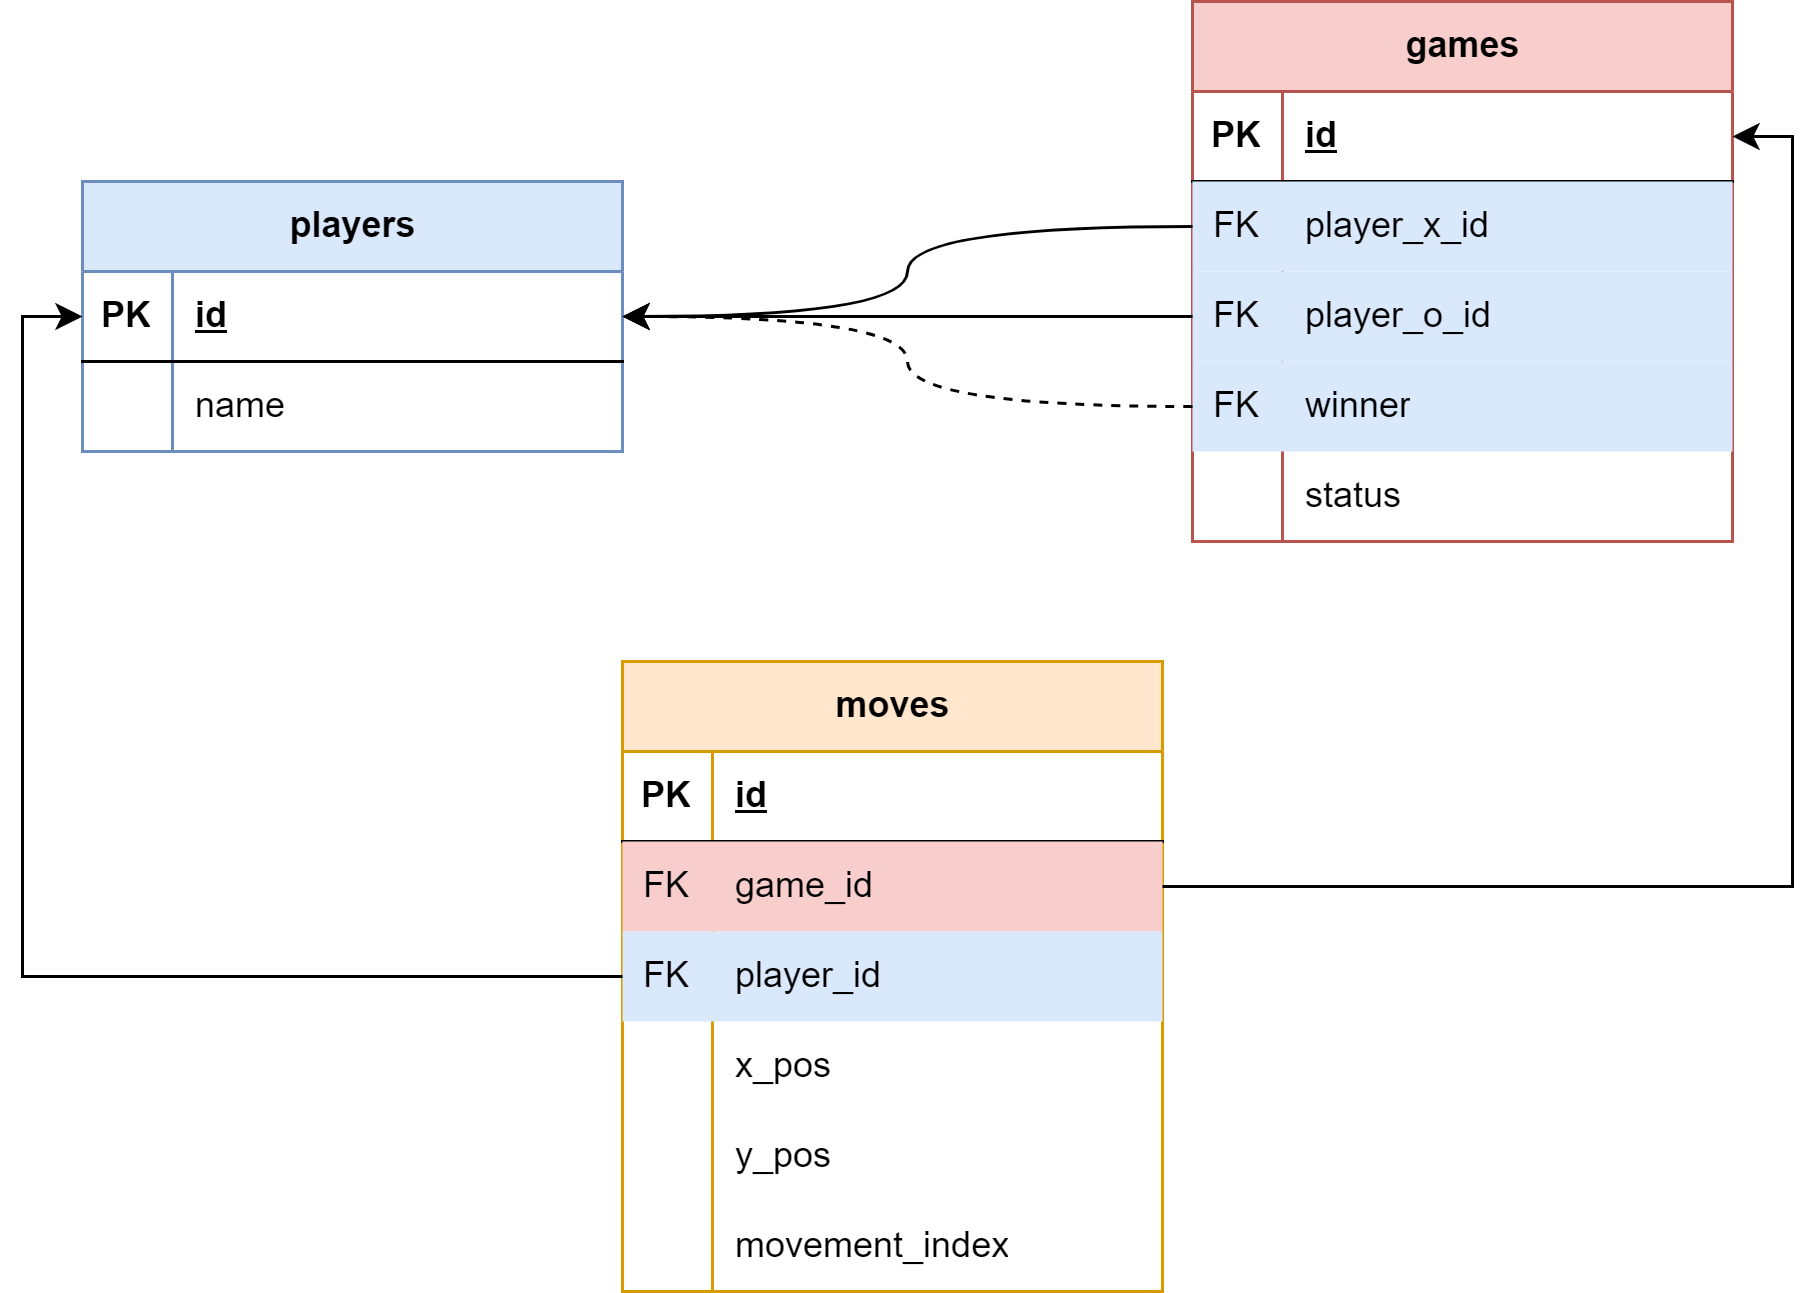
\includegraphics[width=1\textwidth]{tictactoe_mcd.png}
    \caption{Modèle Conceptuel de Données - Morpion}
\end{figure}

{\large \textbf{Pour toutes les questions ci-dessous, referez-vous au MCD du morpion, ainsi qu'a l'annexe.}}

\subsection*{17. Quelles commandes SQL pour créer la table game? /2}
\begin{choices}
  \item \hspace{1cm} \begin{lstlisting}[language=SQL]
    CREATE TABLE games (
        id UUID PRIMARY KEY DEFAULT uuid_generate_v4(),
        player_x_id UUID NOT NULL REFERENCES players(id),
        player_o_id UUID NOT NULL REFERENCES players(id),
        winner UUID REFERENCES players(id) NULL,
        status TEXT CHECK (status IN ('ongoing', 'finished')) NOT NULL
      );
  \end{lstlisting}

  \item \hspace{1cm} \begin{lstlisting}[language=SQL]
      CREATE TABLE games (
        id UUID PRIMARY KEY DEFAULT uuid_generate_v4(),
        player_x_id UUID NOT NULL,
        player_o_id UUID NOT NULL,
        winner UUID NULL,
        status TEXT CHECK (status IN ('ongoing', 'finished')) NOT NULL
      );
      ALTER TABLE games
      ADD CONSTRAINT games_player_x_id_fkey FOREIGN KEY (player_x_id) REFERENCES players(id);

      ALTER TABLE games
      ADD CONSTRAINT games_player_o_id_fkey FOREIGN KEY (player_o_id) REFERENCES players(id);

      ALTER TABLE games
      ADD CONSTRAINT games_winner_fkey FOREIGN KEY (winner) REFERENCES players(id);

  \end{lstlisting}

  \item \hspace{1cm} \begin{lstlisting}[language=SQL]
      CREATE TABLE games (
        id UUID PRIMARY KEY,
        player_x_id UUID NOT NULL,
        player_o_id UUID NOT NULL,
        winner UUID NULL,
        status TEXT CHECK (status IN ('ongoing', 'finished')) NOT NULL
      );
  \end{lstlisting}

  \item \hspace{1cm} \begin{lstlisting}[language=SQL]
      CREATE TABLE games (
        id STRING PRIMARY KEY,
        player_x_id STRING NOT NULL,
        player_o_id STRING NOT NULL,
        winner STRING NULL,
        status TEXT CHECK (status IN ('ongoing', 'finished')) NOT NULL
      );
  \end{lstlisting}

  \item \hspace{1cm} \begin{lstlisting}[language=SQL]
      CREATE TABLE games (
        id UUID PRIMARY KEY DEFAULT uuid_generate_v4(),
        player_x_id UUID NOT NULL REFERENCES players(id),
        player_o_id UUID NOT NULL REFERENCES players(id),
        winner UUID REFERENCES players(id) NULL
      );
  \end{lstlisting}
\end{choices}

\subsection*{18. Quelles tables ne contient pas directement d'information sur les positions (x et y) d'un mouvement dans un jeu ? /1}
\begin{choices}
    \item players
    \item games
    \item moves
\end{choices}

\subsection*{19. Quelles contraintes garantit qu'un mouvement est associé à un jeu spécifique ? /1}
\begin{choices}
    \item game\_id UUID NOT NULL
    \item UNIQUE (game\_id, movement\_index)
    \item id UUID PRIMARY KEY DEFAULT uuid\_generate\_v4()
    \item x\_pos INTEGER NOT NULL
\end{choices}

\subsection*{20. Est-il possible pour un jeu d'avoir le même joueur comme `player\_x` et `player\_o` ? /1}
\begin{choices}
    \item Oui, car il n'y a aucune contrainte empêchant cela.
    \item Non, car il y a une contrainte `CHECK` empêchant cela.
    \item Oui, mais seulement si le champ `winner` est NULL.
    \item Non, car un joueur ne peut jouer qu'une seule fois.
\end{choices}

\subsection*{21. Dans la table `games`, quelle est la contrainte imposée sur le champ `status` ? /1}
\begin{choices}
    \item Le champ `status` doit être soit 'ongoing', soit 'finished'.
    \item Le champ `status` doit être soit 'player\_x', soit 'player\_o'.
    \item Le champ `status` doit être un UUID valide.
    \item Il n'y a pas de contrainte imposée sur le champ `status`.
\end{choices}

\subsection*{22. Quelle est la fonction de `uuid\_generate\_v4()` dans la définition de la table ? /1}
\begin{choices}
    \item Elle génère un identifiant unique basé sur l'heure actuelle.
    \item Elle génère un nombre aléatoire entre 1 et 4.
    \item Elle génère un identifiant unique basé sur l'adresse IP du serveur.
    \item Elle génère un identifiant unique sous forme d'UUID version 4.
\end{choices}

\newpage

\subsection*{23. Quelle requête SQL permet d'obtenir le nom du joueur `X` et du joueur `O` pour chaque jeu enregistré dans la table `games` ? /1}
\begin{choices}
    \item \hspace{1cm}
    \begin{lstlisting}[language=SQL]
    SELECT p1.name, p2.name
    FROM games
    JOIN players p1 ON games.player_x_id = p1.id
    JOIN players p2 ON games.player_o_id = p2.id;
    \end{lstlisting}

    \item \hspace{1cm}
    \begin{lstlisting}[language=SQL]
    SELECT player_x_id, player_o_id FROM games;
    \end{lstlisting}

    \item \hspace{1cm}
    \begin{lstlisting}[language=SQL]
    SELECT name FROM players WHERE id IN (SELECT player_x_id, player_o_id FROM games);
    \end{lstlisting}

    \item \hspace{1cm}
    \begin{lstlisting}[language=SQL]
    SELECT name FROM players
    JOIN games ON players.id = games.player_x_id
    OR players.id = games.player_o_id;
    \end{lstlisting}
\end{choices}

\newpage
\subsection*{24. Si on souhaite créer une vue `v\_active\_games` qui liste tous les jeux en cours (`status` égal à 'ongoing') avec les noms des joueurs, quelle serait la requête SQL appropriée ? /2}
\begin{choices}
    \item \hspace{1cm}
    \begin{lstlisting}[language=SQL]
    CREATE VIEW v_active_games AS
    SELECT p1.name AS Player_X, p2.name AS Player_O
    FROM games
    JOIN players p1 ON games.player_x_id = p1.id
    JOIN players p2 ON games.player_o_id = p2.id
    WHERE status = 'ongoing';
    \end{lstlisting}

    \item  \hspace{1cm}
    \begin{lstlisting}[language=SQL]
    SELECT p1.name, p2.name
    FROM games
    JOIN players p1 ON games.player_x_id = p1.id
    JOIN players p2 ON games.player_o_id = p2.id
    WHERE status = 'ongoing';
    \end{lstlisting}

    \item  \hspace{1cm}
    \begin{lstlisting}[language=SQL]
    CREATE VIEW v_active_games AS
    SELECT player_x_id, player_o_id
    FROM games
    WHERE status = 'finished';
    \end{lstlisting}

    \item  \hspace{1cm}
    \begin{lstlisting}[language=SQL]
    CREATE TABLE v_active_games AS
    SELECT p1.name, p2.name
    FROM games
    JOIN players p1 ON games.player_x_id = p1.id
    JOIN players p2 ON games.player_o_id = p2.id
    WHERE status = 'ongoing';
    \end{lstlisting}

    \item  \hspace{1cm}
    \begin{lstlisting}[language=SQL]
    SELECT * FROM v_active_games
    WHERE status = 'ongoing';
    \end{lstlisting}
\end{choices}

\subsection*{25. Qu'est-ce qu'une window function en SQL? /1}
\begin{choices}
    \item Une fonction qui ouvre une nouvelle fenêtre dans l'interface utilisateur de la base de données.
    \item Une fonction qui permet d'effectuer des calculs sur un ensemble de lignes de table qui sont d'une certaine manière liées à la ligne courante, sans changer la cardinalité du résultat.
    \item Une fonction qui permet d'appliquer une transformation graphique à l'affichage des données, telle qu'une fenêtre pop-up.
    \item Une fonction qui limite le nombre de résultats retournés par une requête à une fenêtre de temps spécifique.
    \item Une fonction qui active le mode "fenêtre" de la base de données, offrant une interface utilisateur améliorée.
\end{choices}

\subsection*{26. Quelle est la fonction principale de l'opérateur `GROUP BY` en SQL? /1}
\begin{choices}
    \item Regrouper les résultats d'une requête par une ou plusieurs colonnes pour permettre des agrégations comme `SUM`, `AVG`, etc.
    \item Trier les résultats d'une requête en fonction de l'ordre alphabétique ou numérique d'une colonne.
    \item Filtrer les résultats d'une requête en fonction d'une condition spécifiée.
    \item Joindre deux tables ou plus en se basant sur une ou plusieurs colonnes communes.
    \item Dupliquer les lignes d'une table en fonction d'une colonne spécifiée.
\end{choices}

\subsection*{27. Quelle est la syntaxe correcte pour ordonner les résultats d'une requête SQL en fonction de la colonne `name` dans un ordre décroissant? /2}
\begin{choices}
    \item SELECT * FROM players ORDER BY name DESC;
    \item SELECT * FROM players SORT BY name DESCENDING;
    \item SELECT * FROM players ORDER name DESC;
    \item SELECT * FROM players WHERE ORDER BY name DESC;
    \item SELECT * FROM players SORT BY name DESC;
    \item SELECT * FROM players ORDER BY name DESCENDING;
\end{choices}

\newpage
\subsection*{28. Considérez les données suivantes dans la table employees: /2}

\begin{table}[h]
    \centering
    \begin{tabular}{|c|c|c|c|}
    \hline
    \textbf{id} & \textbf{name} & \textbf{birth\_date} & \textbf{salary} \\
    \hline
    1 & Alice & 1990-02-15 & 5000 \\
    2 & Bob & 1985-10-23 & 6000 \\
    3 & Charlie & 1995-05-28 & 4500 \\
    4 & David & 1992-11-14 & 6200 \\
    5 & Eve & 1993-04-03 & 5700 \\
    \hline
    \end{tabular}
\end{table}


\textbf{Quelle requête retourne le nombre total d'employés et le salaire moyen, ainsi que le nom de l'employé le plus âgé et le plus jeune (en fonction de la date de naissance) ?}

\begin{choices}
\item \hspace{1cm}\begin{lstlisting}[language=SQL]
SELECT COUNT(id) as Total_Employees, AVG(salary) as Average_Salary,
MAX(name) OVER (ORDER BY birth_date ASC) as Oldest_Employee,
MIN(name) OVER (ORDER BY birth_date DESC) as Youngest_Employee
FROM employees;
\end{lstlisting}
\item \hspace{1cm}\begin{lstlisting}[language=SQL]
SELECT COUNT(id) as Total_Employees, AVG(salary) as Average_Salary,
name WHERE birth_date = MIN(birth_date),
name WHERE birth_date = MAX(birth_date)
FROM employees;
\end{lstlisting}
\item \hspace{1cm}\begin{lstlisting}[language=SQL]
SELECT COUNT(id) as Total_Employees, AVG(salary) as Average_Salary,
FIRST_VALUE(name) OVER (ORDER BY birth_date ASC) as Oldest_Employee,
FIRST_VALUE(name) OVER (ORDER BY birth_date DESC) as Youngest_Employee
FROM employees;
\end{lstlisting}
\item \hspace{1cm}\begin{lstlisting}[language=SQL]
SELECT COUNT(id) as Total_Employees, SUM(salary)/COUNT(id) as Average_Salary,
MAX(name) FROM employees WHERE birth_date = MIN(birth_date),
MAX(name) FROM employees WHERE birth_date = MAX(birth_date)
FROM employees;
\end{lstlisting}
\end{choices}

\newpage
\appendix
\section{Annexe : Schéma de la base de données}

\begin{lstlisting}[style=terminalStyle]
tictactoe=# \d players
    Table "public.players"
Column | Type | Collation | Nullable |      Default
--------+------+-----------+----------+--------------------
id     | uuid |           | not null | uuid_generate_v4()
name   | text |           | not null |
Indexes:
"players_pkey" PRIMARY KEY, btree (id)
Referenced by:
TABLE "games" CONSTRAINT "games_player_o_id_fkey" FOREIGN KEY (player_o_id) REFERENCES players(id)
TABLE "games" CONSTRAINT "games_player_x_id_fkey" FOREIGN KEY (player_x_id) REFERENCES players(id)
TABLE "games" CONSTRAINT "games_winner_fkey" FOREIGN KEY (winner) REFERENCES players(id)

tictactoe=# \d games
        Table "public.games"
Column    | Type | Collation | Nullable |      Default
-------------+------+-----------+----------+--------------------
id          | uuid |           | not null | uuid_generate_v4()
player_x_id | uuid |           | not null |
player_o_id | uuid |           | not null |
winner      | uuid |           |          |
status      | text |           | not null |
Indexes:
"games_pkey" PRIMARY KEY, btree (id)
Check constraints:
"games_status_check" CHECK (status = ANY (ARRAY['ongoing'::text, 'finished'::text]))
Foreign-key constraints:
"games_player_o_id_fkey" FOREIGN KEY (player_o_id) REFERENCES players(id)
"games_player_x_id_fkey" FOREIGN KEY (player_x_id) REFERENCES players(id)
"games_winner_fkey" FOREIGN KEY (winner) REFERENCES players(id)
Referenced by:
TABLE "moves" CONSTRAINT "moves_game_id_fkey" FOREIGN KEY (game_id) REFERENCES games(id)

tictactoe=# \d moves
           Table "public.moves"
Column     |  Type   | Collation | Nullable |      Default
----------------+---------+-----------+----------+--------------------
id             | uuid    |           | not null | uuid_generate_v4()
game_id        | uuid    |           | not null |
x_pos          | integer |           | not null |
y_pos          | integer |           | not null |
movement_index | integer |           | not null |
Indexes:
"moves_pkey" PRIMARY KEY, btree (id)
"moves_game_id_movement_index_key" UNIQUE CONSTRAINT, btree (game_id, movement_index)
Foreign-key constraints:
"moves_game_id_fkey" FOREIGN KEY (game_id) REFERENCES games(id)
\end{lstlisting}


\end{flushleft}
\end{document}
